\documentclass[12pt,twoside,a4paper,notitlepage]{report}

\setlength{\oddsidemargin}{2mm}
\setlength{\evensidemargin}{2mm}
\setlength{\textwidth}{154mm}
\setlength{\textheight}{220mm}
\setlength{\topmargin}{0mm}
\setlength{\parskip}{1mm}
\renewcommand{\floatpagefraction} {0.99}
\renewcommand{\textfraction} {0.0}
\renewcommand{\topfraction} {0.99}

\renewcommand{\baselinestretch}{1.1}

\vbadness=10001 % the hell with underfull vboxes
\hbadness=10001

%\usepackage[latin2]{inputenc}
\usepackage{fancyhdr}
%\usepackage{makeidx}
\usepackage{amssymb}
\usepackage{url}
\usepackage{longtable}
\usepackage{multicol}
\usepackage{graphics}
\usepackage{graphicx} 
\usepackage{subfigure}
\usepackage{pslatex}
\usepackage{multirow}
\usepackage{fancyvrb}
\usepackage{xcolor}
\usepackage{siunitx}
\usepackage[colorlinks=true, pdfstartview=FitV, linkcolor=blue, 
	    citecolor=blue, urlcolor=blue]{hyperref}

\pagestyle{fancy}

\addtolength{\headheight}{\baselineskip}

\renewcommand{\chaptermark}[1]{\markboth{\chaptername \ \thechapter.\ #1}{}}
\renewcommand{\sectionmark}[1]{\markright{\thesection.\ #1}}

\newcommand{\clearemptydoublepage}{\newpage{\pagestyle{empty}\cleardoublepage}}

\setcounter{secnumdepth}{5}

\newcommand{\Lletterstyle}[1]{%
  \textcolor{red}{\textbf{#1}}%
}
\DeclareRobustCommand{\BLaTeX}{\Lletterstyle{L}\kern-.35em%
  {\sbox\z@ T%
    \vbox to\ht\z@{\hbox{\check@mathfonts
        \fontsize\sf@size\z@
        \math@fontsfalse\selectfont
        A}%
      \vss}%
  }%
  \kern-.15em%
  \TeX%
}
\DeclareRobustCommand{\BLaTeXe}{\mbox{\m@th
  \if b\expandafter\@car\f@series\@nil\boldmath\fi
  \BLaTeX\kern.15em2$_{\textstyle\varepsilon}$}}
\makeatother

\makeatletter
\newcommand*{\toccontents}{\@starttoc{toc}}
\makeatother

\begin{document} 

%\newcommand{\helv}{%
% \fontfamily{phv}\fontseries{b}\fontsize{9}{11}\selectfont}

\fancyhf{}

\fancyhead{} % clear all fields
\fancyhead[LO]{\rightmark }
\fancyhead[RE]{\leftmark }
\fancyhead[LE,RO]{\thepage }
%\fancyfoot[CO,CE]{\thepage }

\title{\textbf{thermal processing panel} - an overview}
\author{author: Petre Rodan}
\date{revised \today}
\maketitle
%\tableofcontents
\toccontents

\chapter{GUI elements}

\section{overview}

sub-windows (or panels) are enabled via the main menu. once opened they can be dragged even outside of the main program area or docked into pre-defined positions. for further details see \href{https://github.com/ocornut/imgui/wiki/Docking}{the imgui wiki}. this provides a lot of flexibility in determining optimal screen use.

the main viewport window can never be closed and it shows either the currently processed image or a highlight overlay. the thermal image itself is basically an array of temperatures displayed in fake colors picked from a palette.

hovering the mouse over the image will show the compensated temperature in that point, the scrollwheel pans the image vertically (if the viewport is too small),  pressing SHIFT while scrolling pans the image horizontally. pressing CTRL while using the scrollwheel zooms in and out. clicking and dragging is context-sensitive and generates an overlay highlight  (see section \ref{sec:tools-export}).

the general feel and the text scaling can be changed via the theme selector (see section \ref{sec:tools-preferences})

properties of interest can be selected in the preferences panel \ref{sec:tools-preferences} and then displayed by enabling the file/properties panel.

all the constants that contribute to the calculated compensated temperature can be tweaked in the processing panel (see \ref{sec:tools-processing}).

most panels can be closed either via the main menu or by pressing the upper-right 'x' button.

\newpage

\section{file library} \label{sec:file-library}

an embedded file explorer window that renders all supported thermal images as thumbnails. these thumbnails are generated on-the-fly when a directory is opened and are cached for the lifetime of the thpp process. multiple threads are used to render them in order to minimize the processing time.

the filesystem entries are refreshed every few seconds, so if a new image is copied into the currently-open directory it will show up automatically. double-clicking any of images will open the thermogram in the viewport, double-clicking on the folder icons will change the working directory.

in the preferences window the thumbnail size and the palette can be customized, but the palette setting only applies to images that have not been cached yet.

\begin{figure}[ht]
 \centering
 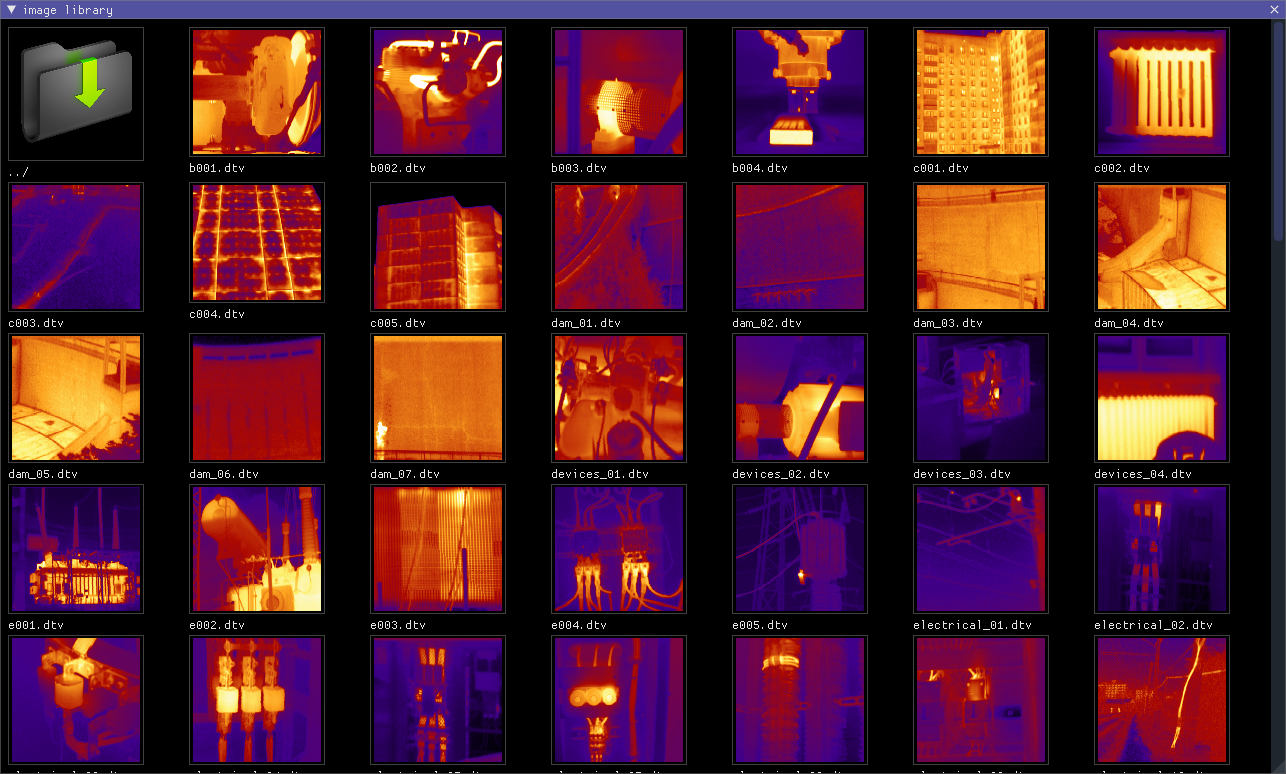
\includegraphics[width=14cm, keepaspectratio=true]{img/file_library}
 \caption{file library panel}
 \label{fig:file-library-overview}
\end{figure}

\section{scale tool} \label{sec:tools-scale}

the scale provides the equivalence function between the palette colors and the compensated temperature. a printed thermal image without this scale provides little to no information.

instead of craming the scale into the image space, a separate exportable image is created for it. the tick marks are generated automatically at round values. their color always stand out from the palette. the number of major and minor ticks is determined automatically based on the temperature interval.

\begin{figure}[ht]
 \centering
 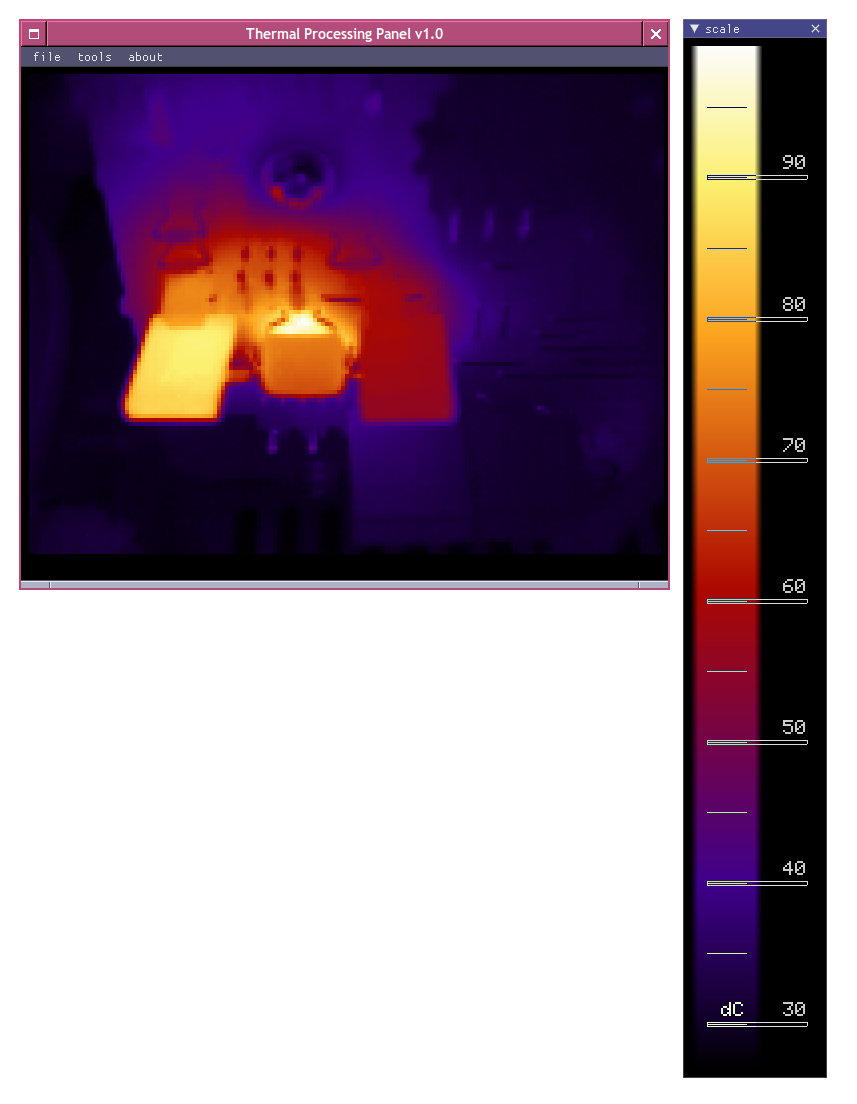
\includegraphics[width=6cm, keepaspectratio=true]{img/tools_scale}
 \caption{tools/scale panel as visible in thpp}
 \label{fig:tools-scale}
\end{figure}

\begin{figure}[ht]
 \centering
 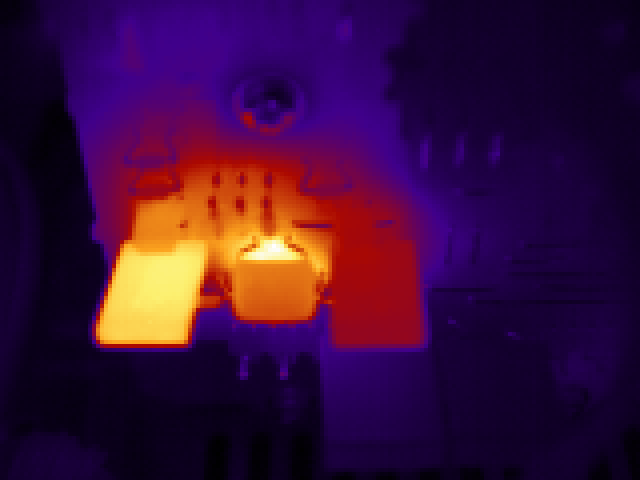
\includegraphics[width=10cm, keepaspectratio=true]{img/tools_scale_exported}
 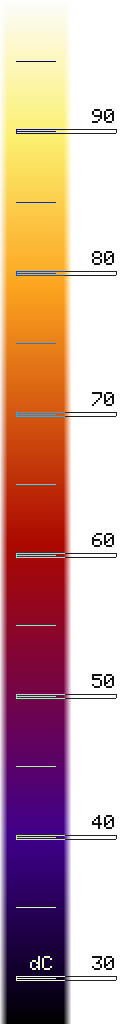
\includegraphics[width=9.5mm, keepaspectratio=true]{img/tools_scale_exported_scale}
 \caption{exported scale and image}
 \label{fig:tools-scale-exported}
\end{figure}

\newpage

\section{processing tool} \label{sec:tools-processing}

the temperature array that constitutes the thermal image is obtained by feeding an array of raw ADC samples into a function that takes into acount the distance between the object and camera, the surface emissivity, atmospheric conditions, camera optics and camera calibration values. most of these constants (except the camera calibration) can be tweaked to better reflect the conditions in which the image was taken. the higher the accuracy of the input constants the more likely the compensated output temperature reflects reality.

by far the most important constant that needs to be precisely provided is the emissivity. make sure to consult an emissivity table to enter the proper value depending on the surface texture and material of the object that was captured in the image.

the palette is an array of fake colors that is used to convey the temperature values in a meaningful way. internally each palette is generated over a 16bit space (so that up to $2^{16}$ unique colors can be assigned to the temperature values present in an image). \href{https://inkscape.org/}{inkscape} can be used to create new palettes (see the \href{https://github.com/rodan/thpp/blob/main/palette/hmetal2.svg}{svg sample} files). an svg-to-C converter \href{https://github.com/rodan/thpp/blob/main/palette/extract_pal.sh}{bash script} is also provided.

a rescale of the temperature limits is also possible if the same palette color has to reflect the same temperature over a set of images. useful for creating panoramas or reports.


\begin{figure}[ht]
 \centering
 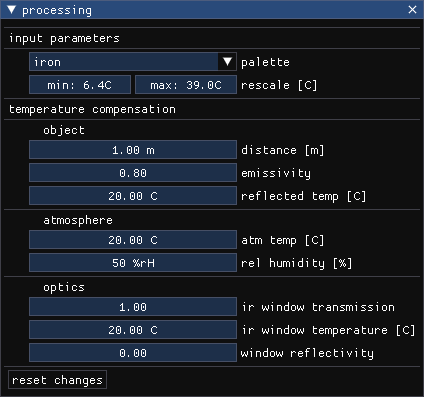
\includegraphics[width=6cm, keepaspectratio=true]{img/tools_processing}
 \caption{tools/processing panel}
 \label{fig:tools-processing}
\end{figure}

\section{histogram and line profile tools} \label{sec:tools-histogram}

once an image is opened, it's temperature distribution can be visualized in a histogram. the number of bins is configurable.

\begin{figure}[ht]
 \centering
 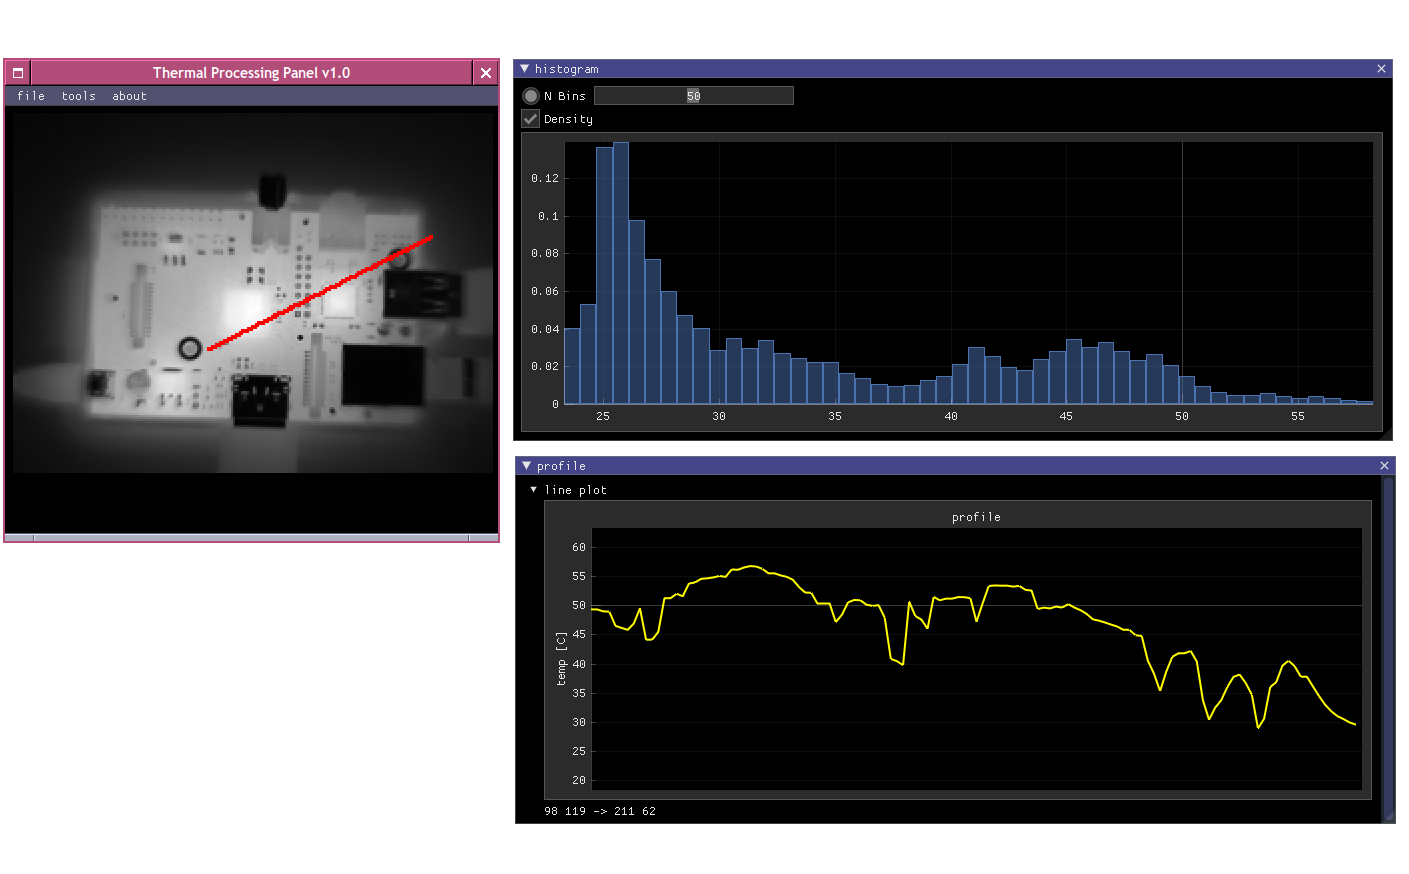
\includegraphics[width=11cm, keepaspectratio=true]{img/tools_histogram}
 \caption{histogram and line profile panels}
 \label{fig:tools-histogram}
\end{figure}


a profile line can be defined in the tools/export panel by following the steps below:
\begin{itemize}
    \item open tools/export
    \item enable highlight layer
    \item activate preview
    \item profile type - line
    \item press pick line
    \item click (LMB) on the image to establish the first point of the line
    \item while still pressing LMB drag the pointer to the second point of the line
    \item release LMB to confirm the second point
\end{itemize}

if the line itself lacks contrast against the neighboring pixels, the default highlight color can be switched from palette-based to a solid red color.


\section{preferences} \label{sec:tools-preferences}

this panel changes the look and feel of thpp. the color theme can be picked, the gui font scale (select 2 for HiDPI displays), size of the library image thumbnails, the zoom level and algorithm of the image. two interpolation algorithms have been implemented. nearest-neighbor which simply duplicates pixels horizontally using the same value as the last encountered pixel and vertically by repeating the last line from the image. this is a very fast algorithm that keeps most of the information intact without adding noise but it does produce jagged edges at some angles. the second one, called \href{https://github.com/xinntao/Real-ESRGAN}{Real-ESRGAN} is the exact opposite.

Note. make sure the image is zoomed in with 'nearest' interpolation while applying new temperature compensation values or defining a line profile. realsr's extremely heavy GPU algorithm is not suited for real-time updates of the zoomed image. 

\begin{figure}[ht]
 \centering
 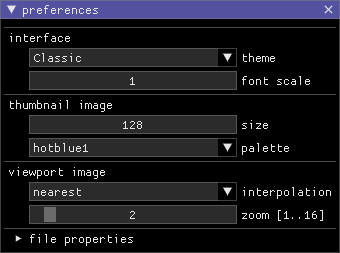
\includegraphics[width=5cm, keepaspectratio=true]{img/tools_preferences}
 \caption{preferences panel}
 \label{fig:tools-preferences}
\end{figure}

\begin{figure}[ht]
 \centering
 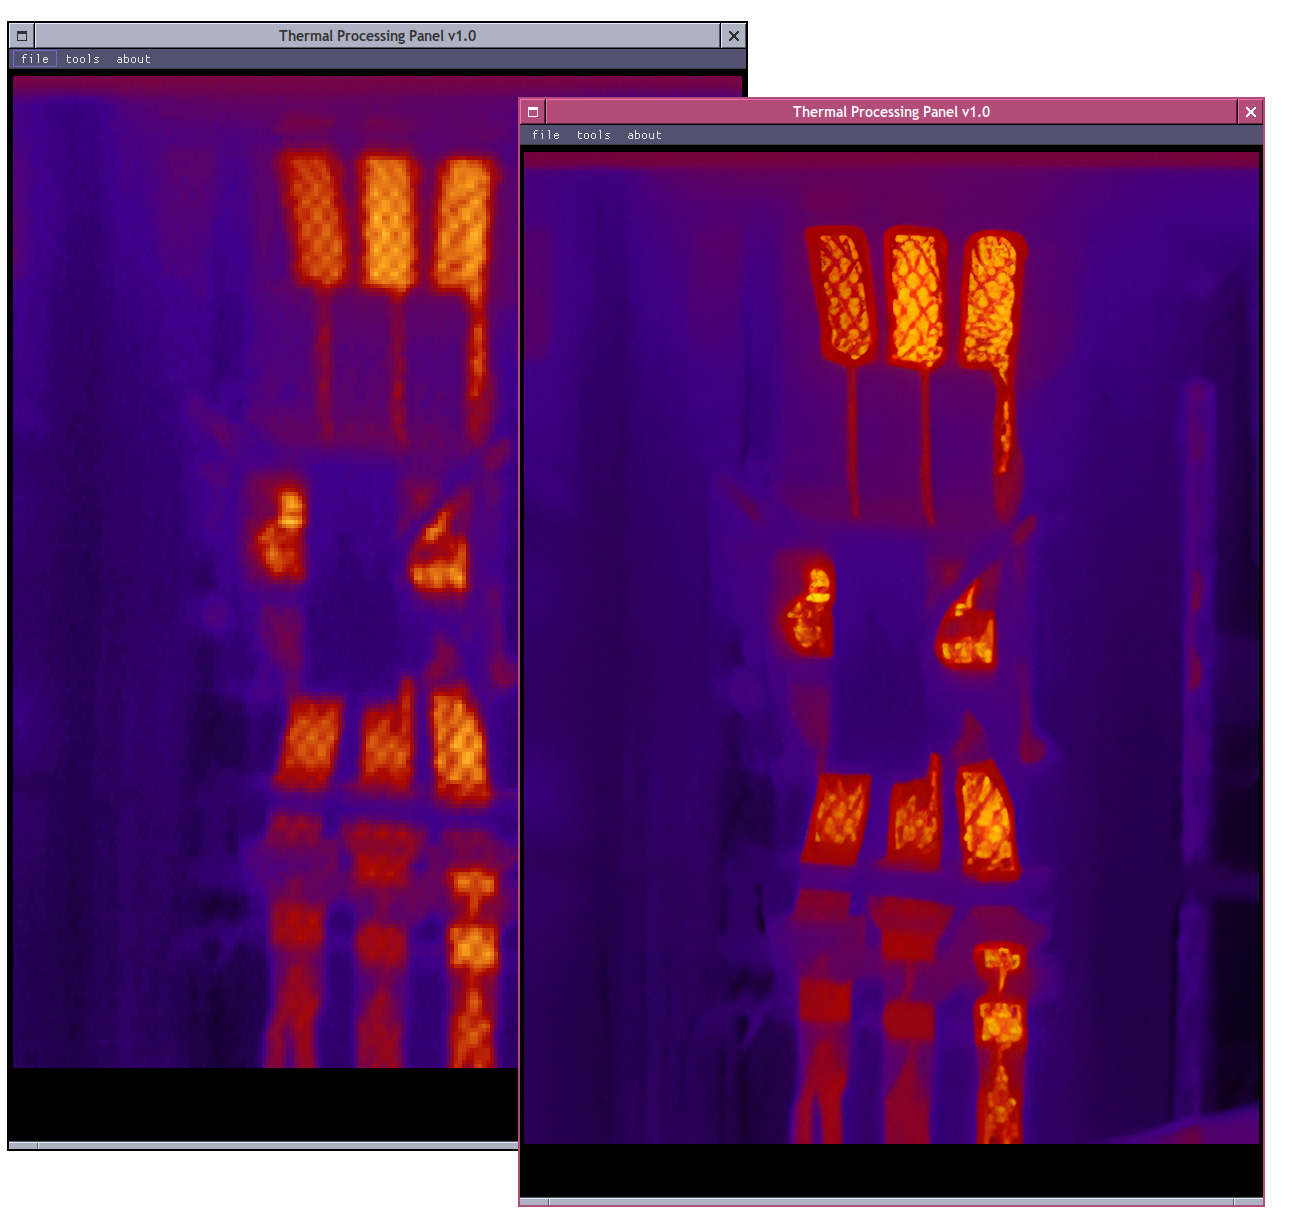
\includegraphics[width=14cm, keepaspectratio=true]{img/zoom_interpolation}
 \caption{4x interpolation comparison: nearest-neighbor (left) vs realsr (on the right)}
 \label{fig:relasr interpolation}
\end{figure}


\section{file properties} \label{sec:file-properties}

a customizable set of file properties can be displayed once enabling the panel with the same name.

the customization of which elements should be shown is done via the tools/preferences panel (see section \ref{sec:tools-preferences}). these vary from camera model, calibration constants to min/max/avg values obtained after calculating the compensated temperature array. some are camera or even file format specific so they might remain invisible in the output table.

the exact same set of elements can also be exported into a \LaTeX \ compatible text file (see section \ref{sec:tools-export}).

\begin{figure}[ht]
 \centering
 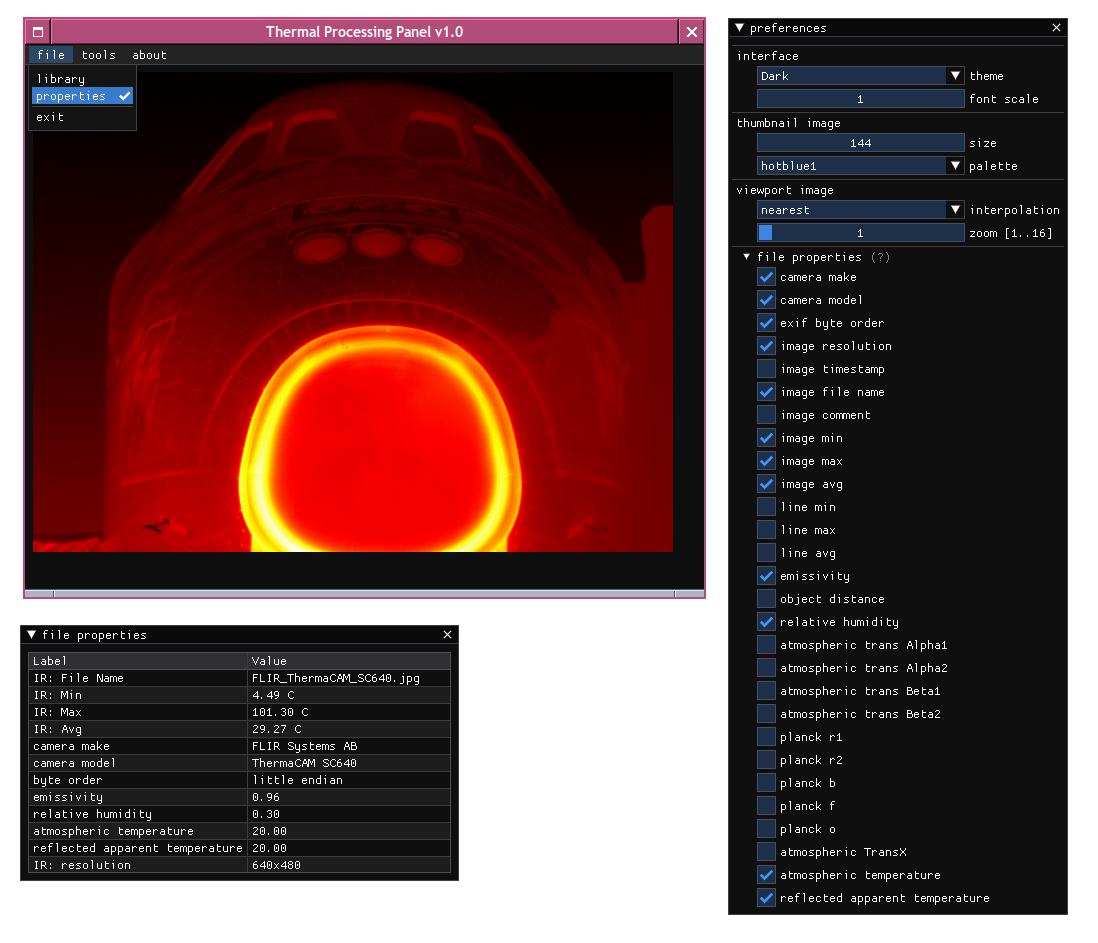
\includegraphics[width=14cm, keepaspectratio=true]{img/file_properties}
 \caption{file properties panel}
 \label{fig:file-properties-overview}
\end{figure}


\section{export tool} \label{sec:tools-export}

the export tool provides a highlight feature in which certain zones of a thermal image can be displayed in a more prominent manner.

the effect is achieved by rendering the thermogram using a gray palette and using either the current palette or a solid color to highlight certain areas. these areas can be selected in a few ways: via a temperature-based level slice technique, by automatically selecting a zone centered around a chosen coordinate or by defining a line profile over the image.

this overlay can to be activated via the 'enable highlight layer' and can be shown and hidden via the 'preview' checkbox. the 'profile type' combo box selects one of the three highlight types mentioned above.

all the 'export ...' buttons generate the output files inside the directory defined by the 'dest directory' textbox. the filenames are created based on the 'prefix' and 'highlight fname' textboxes.

the 'export highlight data' button appears after a profile line has been defined and it produces a gnuplot and a csv file. the idea is to parse the first one with the \href{http://www.gnuplot.info/}{gnuplot} application in order to transform the csv into a graph image.


\begin{figure}[ht]
 \centering
 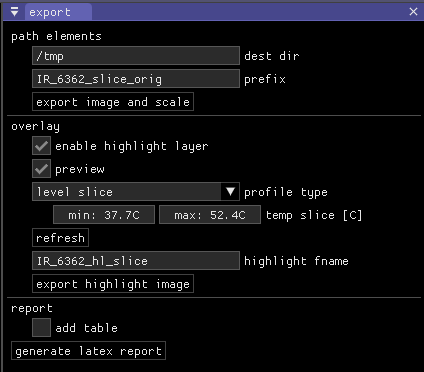
\includegraphics[width=6cm, keepaspectratio=true]{img/tools_export_slice}
 \caption{tools/export panel}
 \label{fig:tools-export-overview}
\end{figure}


\begin{figure}[ht]
 \centering
 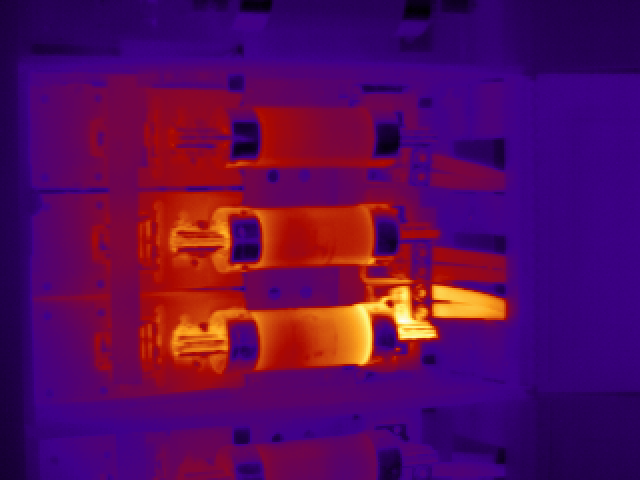
\includegraphics[width=10cm, keepaspectratio=true]{img/FLIR_P60_orig}
 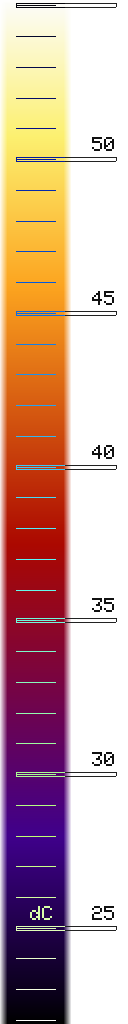
\includegraphics[width=9.5mm, keepaspectratio=true]{img/FLIR_P60_orig_scale}
 \caption{original image - 3 high power fuses in an electrical panel, one of the circuits is overloaded}
 \label{fig:tools-export-orig-image}
\end{figure}


\begin{figure}[ht]
 \centering
 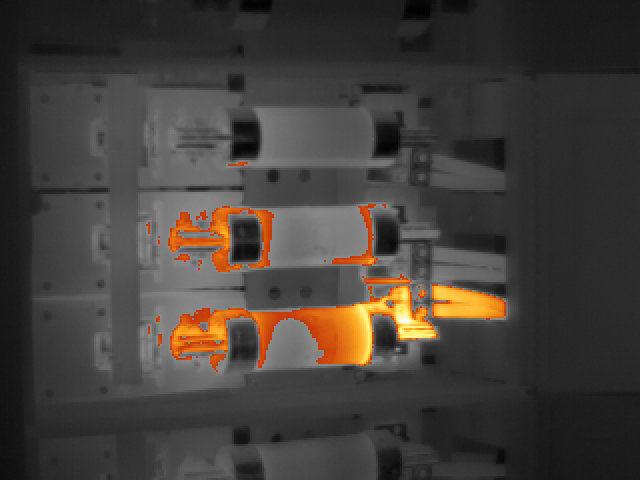
\includegraphics[width=10cm, keepaspectratio=true]{img/FLIR_P60_hl_ls}
 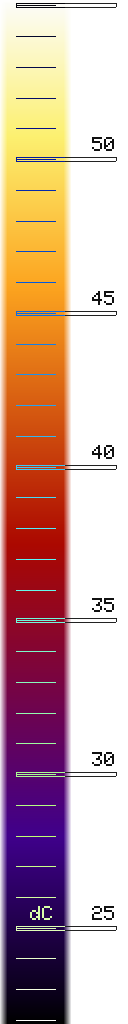
\includegraphics[width=9.5mm, keepaspectratio=true]{img/FLIR_P60_orig_scale}
 \caption{image wide level slice effect - highlights all pixels in a selected temperature interval - in this case everything above 40°C}
 \label{fig:tools-export-level-slice}
\end{figure}

\begin{figure}[ht]
 \centering
 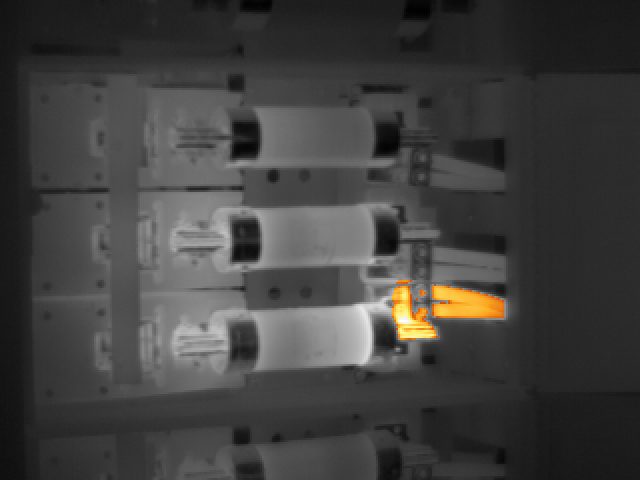
\includegraphics[width=10cm, keepaspectratio=true]{img/FLIR_P60_hl_p}
 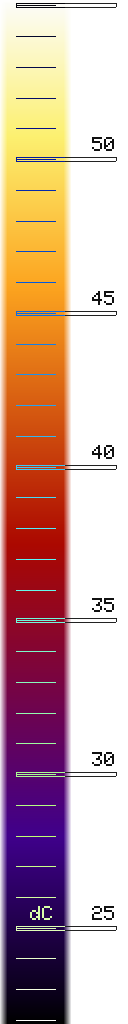
\includegraphics[width=9.5mm, keepaspectratio=true]{img/FLIR_P60_orig_scale}
 \caption{punctiform highlight - overheated cable (31 pixel growth radius, 6 °C max delta)}
 \label{fig:tools-export-punctiform}
\end{figure}


\begin{figure}[ht]
\begin{verbatim}
#!/usr/bin/env gnuplot

plot 'sample_hl.csv' title "" with lines lw 2

set grid y
set grid lc rgb "#dddddd" lt 1
unset xtics
set ylabel '°C' rotate by 0
set terminal png size 1024,300
set output 'sample_hl_gnuplot.png'
set style data lines
replot
\end{verbatim}
\caption{sample gnuplot script generated by the line profile tool}
\end{figure}

\begin{figure}[ht]
 \centering
 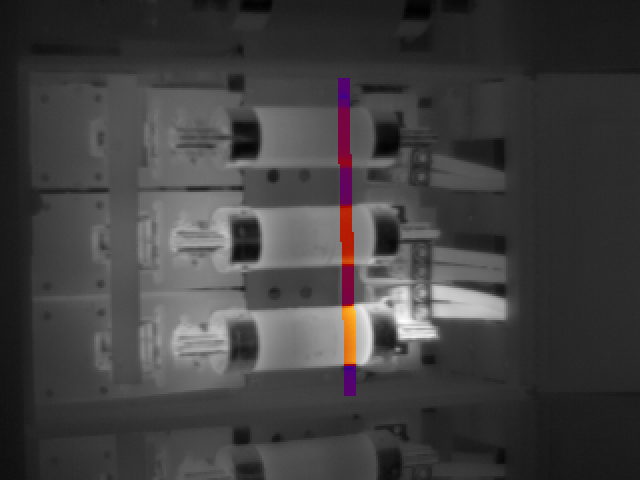
\includegraphics[width=10cm, keepaspectratio=true]{img/FLIR_P60_hl_line}
 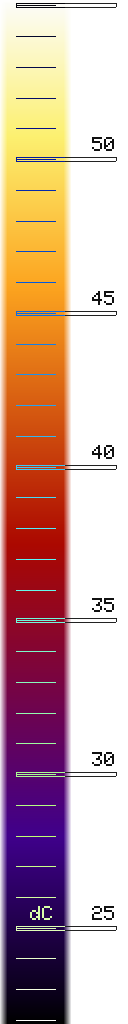
\includegraphics[width=9.5mm, keepaspectratio=true]{img/FLIR_P60_orig_scale}
 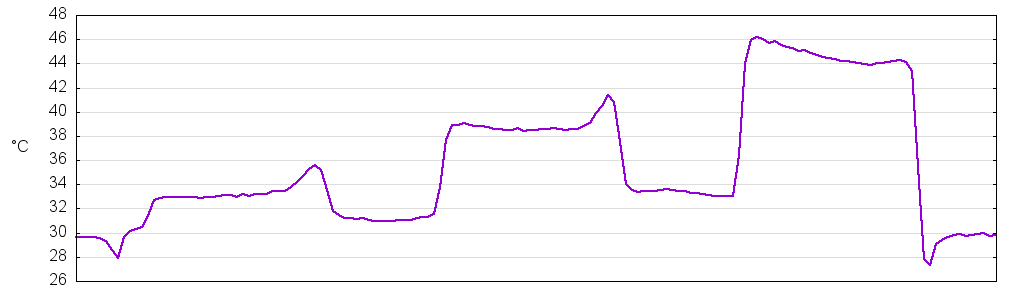
\includegraphics[width=14cm, keepaspectratio=true]{img/FLIR_P60_hl_line_gnuplot}
 \caption{line profile over all 3 fuses and resulting plot}
 \label{fig:tools-export-line}
\end{figure}

\end{document}
